\documentclass{beamer}
\beamertemplatenavigationsymbolsempty 

\title{Bad Graphs}
\subtitle{Healthcare Spending vs. Life Expectancy}

\author{Dustin Ingram}
\institute{STAT601, Summer 12-13\\ Drexel University}
\date{\today}

\begin{document}
\maketitle

\begin{frame}
    \frametitle{A bad graph:}
    \begin{figure}
        \centering
        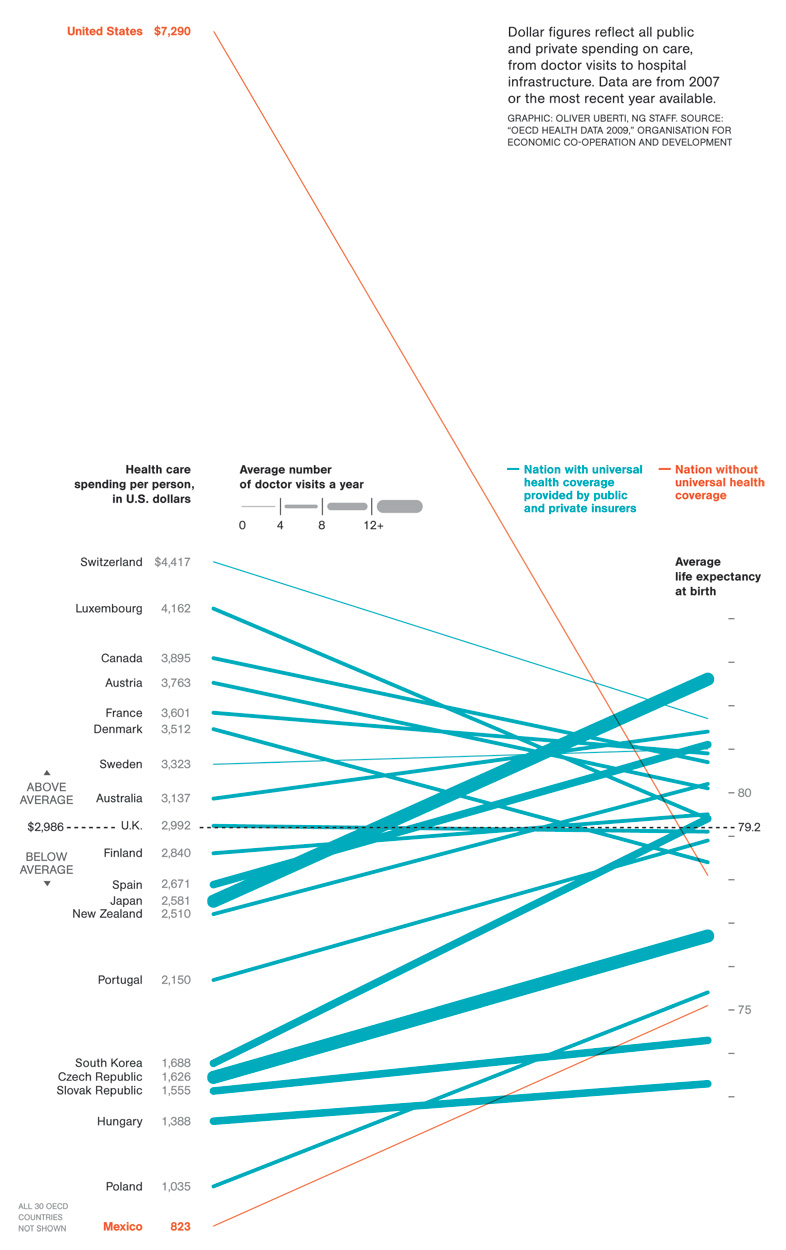
\includegraphics[height=0.8\paperheight]{original.jpg}
    \end{figure}
\end{frame}

\begin{frame}
    \frametitle{So bad, it doesn't even fit\ldots}
    \begin{figure}
        \centering
        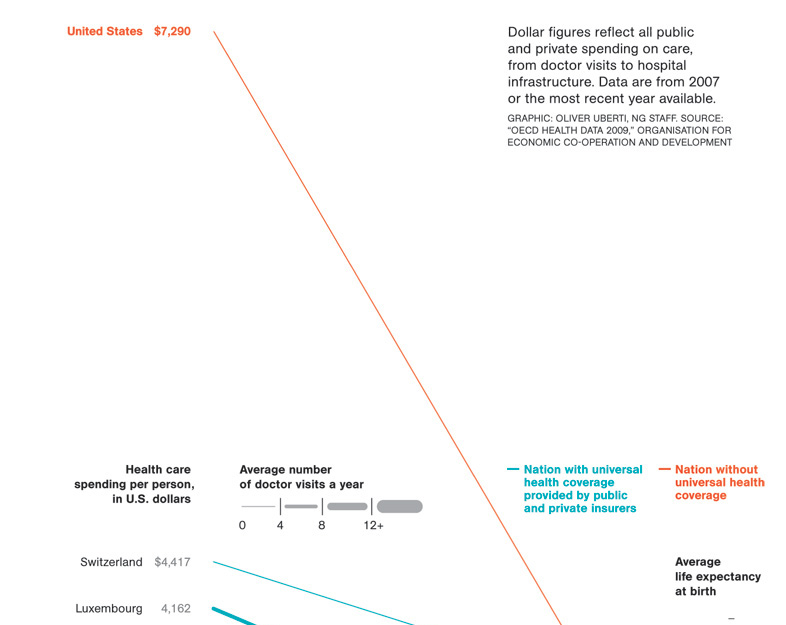
\includegraphics[width=0.8\paperwidth]{top.jpg}
    \end{figure}
\end{frame}

\begin{frame}
    \frametitle{\ldots on one slide.}
    \begin{figure}
        \centering
        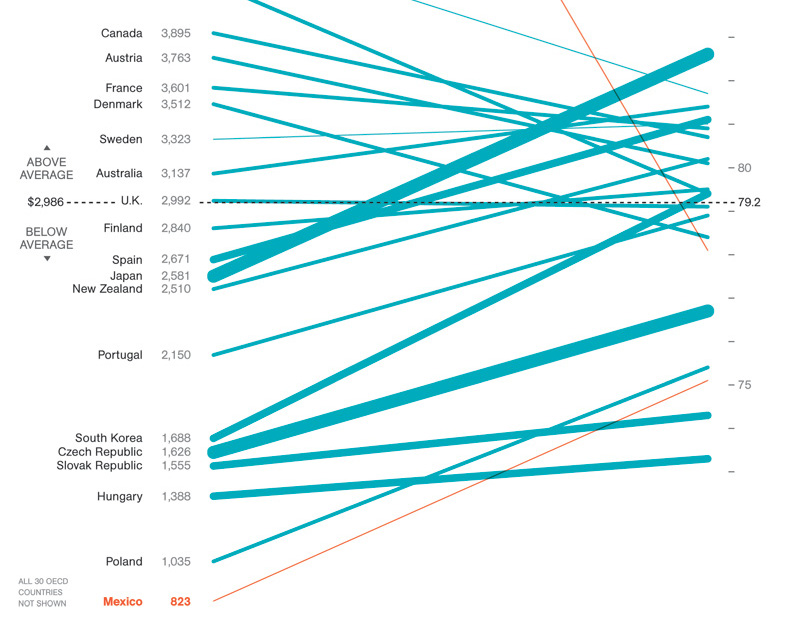
\includegraphics[width=0.8\paperwidth]{bottom.jpg}
    \end{figure}
\end{frame}

\begin{frame}
    \frametitle{Goals of this graph:}
    \begin{itemize}
        \item Show a relationship between average life expectancy and cost of healthcare for each of the OECD (Organisation for Economic Co-operation and Development) member countries;
        \item Show the average life expectancy and cost of healthcare across all of these countries;
        \item Show the average number of doctor consultations per country;
        \item Show which countries have universal healthcare, and which do not;
        \item Show that the United States is an outlier.
    \end{itemize}
\end{frame}

\begin{frame}
    \frametitle{Problems with this graph:}
    \begin{itemize}
        \item Scaling of parallel coordinate plot is arbitrary;
        \item Fails to show correlation between spending and life expectancy;
        \item Is it really necessary to tell the viewer which direction is ``above'' average and which is ``below''?
    \end{itemize}
\end{frame}

{
    \usebackgroundtemplate{\includegraphics[width=\paperwidth,height=\paperheight]{newgraph.pdf}}
    \begin{frame}[plain] \end{frame}
}

\begin{frame}
    \frametitle{Source:}
    \begin{itemize}
        \item 
        %\item http://blogs.ngm.com/blog_central/2009/12/the-cost-of-care.html
        %\item http://web.archive.org/web/20130119003642/http://blogs.ngm.com/blog_central/2009/12/the-cost-of-care.html
        %\item http://web.archive.org/web/20130116193447/http://blogs.ngm.com/.a/6a00e0098226918833012876a6070f970c-800wi
        %\item http://www.oecd.org/els/health-systems/oecdhealthdata2013-frequentlyrequesteddata.htm
    \end{itemize}
\end{frame}

\end{document}
